\chapter{Modello Fisico e Ottimizzazione}

\section*{Introduzione}
Il modello fisico descrive come i dati sono effettivamente memorizzati e organizzati nel disco fisico. Include indici, viste materializzate, partizionamento e altre strategie di ottimizzazione per migliorare performance e scalabilità.

\section*{Obiettivi di apprendimento}
\begin{itemize}
    \item Comprendere come i dati sono memorizzati nel disco
    \item Progettare e utilizzare indici efficaci
    \item Comprendere le viste materializzate e il caching
    \item Applicare strategie di partizionamento
    \item Ottimizzare query e accessi ai dati
    \item Bilanciare velocità di lettura e velocità di scrittura
\end{itemize}

\section{Memorizzazione dei Dati}

\subsection{Struttura di memorizzazione}
I dati vengono memorizzati in una gerarchia ben organizzata all'interno del disco. Un \textbf{blocco} rappresenta l'unità minima di trasferimento tra disco e memoria, tipicamente dimensionato tra 4 e 16 KB per ottimizzare le operazioni di I/O. Una \textbf{pagina} è il corrispondente concetto logico all'interno del DBMS, fungendo da container strutturato dei dati. Un \textbf{record} è la singola tupla della tabella, contenente una riga completa di dati. Infine, un \textbf{campo} rappresenta il singolo attributo di un record, cioè il più piccolo elemento di dato identificabile all'interno della struttura.

\begin{figure}[h]
    \centering
    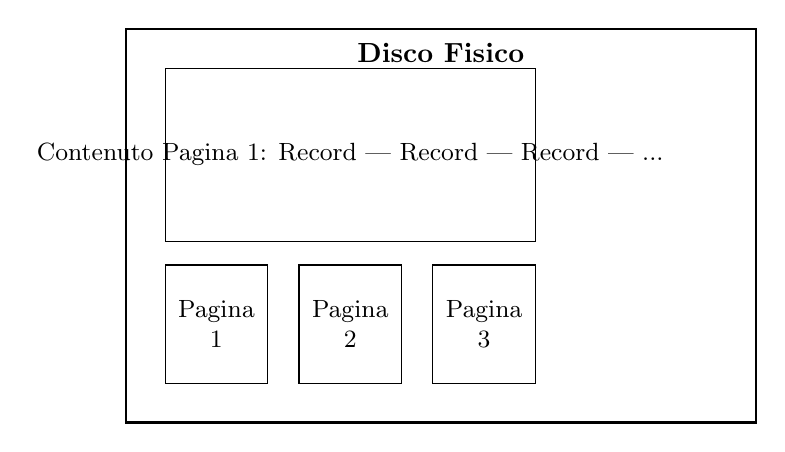
\begin{tikzpicture}[scale=1]
        \draw[thick] (0, 0) rectangle (8, 5);
        \node at (4, 4.7) {\textbf{Disco Fisico}};

        \draw (0.5, 0.5) rectangle (1.8, 2);
        \node[align=center, font=\small] at (1.15, 1.25) {Pagina\\1};

        \draw (2.2, 0.5) rectangle (3.5, 2);
        \node[align=center, font=\small] at (2.85, 1.25) {Pagina\\2};

        \draw (3.9, 0.5) rectangle (5.2, 2);
        \node[align=center, font=\small] at (4.55, 1.25) {Pagina\\3};

        \draw (0.5, 2.3) rectangle (5.2, 4.5);
        \node[align=center, font=\small] at (2.85, 3.4) {Contenuto Pagina 1: Record | Record | Record | ...};
    \end{tikzpicture}
    \caption{Struttura di memorizzazione su disco}
\end{figure}

\subsection{Tipi di accesso}
Esistono due modelli fondamentali di accesso ai dati che differiscono significativamente in termini di efficienza. L'\textbf{accesso sequenziale} implica leggere i record uno dopo l'altro in sequenza, scorrendo l'intera struttura dati. Questo metodo è lento quando si ricerca un record specifico, poiché potrebbe richiedere di esaminare un numero enorme di record prima di trovare quello desiderato. L'\textbf{accesso casuale} consente invece di accedere direttamente a un record specifico senza doverne leggere altri, risultando molto più veloce; tuttavia, questa velocità richiede la disponibilità di strutture ausiliarie come gli indici che guidano il DBMS direttamente al dato cercato.

\section{Indici}

Un \textbf{indice} è una struttura dati che accelera il recupero di record da una tabella. Funziona come un indice di un libro: invece di leggere tutte le pagine, consulti l'indice per trovare la pagina che cerchi.

\subsection{Vantaggi degli indici}
Gli indici offrono benefici significativi per le operazioni di lettura. Accelerano notevolmente le ricerche e i filtri espressi nelle clausole WHERE, permettendo al DBMS di localizzare rapidamente i record corrispondenti. Accelerano anche gli ordinamenti (ORDER BY), poiché gli indici mantengono i dati in ordine predeterminato. Gli indici ottimizzano inoltre le operazioni di join tra tabelle, facilitando l'abbinamento veloce di record correlati. Infine, supportano query range dove è necessario recuperare intervalli di valori, come nella clausola WHERE prezzo BETWEEN 10 AND 100.

\subsection{Svantaggi degli indici}
Nonostante i vantaggi, gli indici comportano anche costi significativi. Occupano spazio aggiuntivo considerevole su disco, aumentando i requisiti di storage. Più criticamente, ralentano le operazioni di INSERT, UPDATE e DELETE, poiché l'indice deve essere aggiornato ogni volta che i dati sottostanti cambiano. Inoltre, gli indici richiedono manutenzione periodica per mantenere l'efficienza, consumando risorse computazionali che potrebbero altrimenti essere dedicate ad altre operazioni.

\subsection{Tipi di indici}

\subsubsection{Indice primario}
Un indice su una chiave primaria. È automaticamente creato quando si definisce una PRIMARY KEY.

\begin{lstlisting}[language=SQL, caption=Indice primario (creato automaticamente)]
CREATE TABLE cliente (
    idCliente INT PRIMARY KEY,  -- Indice primario automatico
    nome VARCHAR(100)
);
\end{lstlisting}

\subsubsection{Indice secondario}
Un indice su attributi non-chiave per accelerare ricerche frequenti.

\begin{lstlisting}[language=SQL, caption=Creare un indice secondario]
CREATE TABLE cliente (
    idCliente INT PRIMARY KEY,
    nome VARCHAR(100),
    email VARCHAR(100),
    città VARCHAR(50)
);

-- Indici su campi frequentemente cercati
CREATE INDEX idx_email ON cliente(email);
CREATE INDEX idx_città ON cliente(città);
\end{lstlisting}

\subsubsection{Indice composito}
Un indice su più attributi, utile per query che filtrano su più colonne.

\begin{lstlisting}[language=SQL, caption=Indice composito]
CREATE TABLE ordine (
    idOrdine INT PRIMARY KEY,
    dataOrdine DATE,
    idCliente INT,
    stato VARCHAR(20)
);

-- Indice su due colonne per query come:
-- WHERE idCliente = 5 AND stato = 'Spedito'
CREATE INDEX idx_cliente_stato ON ordine(idCliente, stato);
\end{lstlisting}

\subsubsection{Indice a hash}
Usa una funzione hash per mappare i valori agli indirizzi di memoria. Veloce per uguaglianza, non per range.

\subsubsection{Indice B-Tree}
La struttura più comune. Ordinato, efficiente per range e ordinamenti. Bilanciato automaticamente.

\begin{lstlisting}[language=SQL, caption=Statistiche dell'indice (MySQL)]
-- Mostra dettagli degli indici di una tabella
SHOW INDEX FROM cliente;

-- Analizza l'efficienza dell'indice
EXPLAIN SELECT * FROM cliente WHERE email = 'mario@email.com';
\end{lstlisting}

\subsection{Strategie di indicizzazione}

\begin{tcolorbox}[colback=green!10, colframe=green!60, title=Buone pratiche per gli indici]
\begin{itemize}
    \item Indicizza campi usati frequentemente in WHERE, JOIN, ORDER BY
    \item Non indicizzare campi usati raramente (spreco di spazio)
    \item Indici compositi per query multi-colonna frequenti
    \item Evita indici su colonne con pochi valori distinti (low cardinality)
    \item Monitora e mantieni gli indici regolarmente
\end{itemize}
\end{tcolorbox}

\section{Viste Materializzate}

Una \textbf{vista materializzata} è il risultato di una query pre-calcolato e memorizzato fisicamente sul disco. A differenza di una vista normale, occupa spazio e deve essere aggiornato.

\subsection{Vantaggi}
Le viste materializzate offrono prestazioni eccezionali per determinati tipi di query. Consentono query estremamente veloci grazie al fatto che i dati sono già pre-calcolati e memorizzati fisicamente, eliminando il bisogno di rielaborazione al momento della richiesta. Riducono significativamente il carico computazionale del DBMS, liberando risorse per altre operazioni. Sono particolarmente utili per query complesse che operano su dati storici, dove i risultati rimangono relativamente stabili nel tempo.

\subsection{Svantaggi}
Nonostante i vantaggi di performance, le viste materializzate presentano limitazioni notevoli. Occupano spazio su disco in modo permanente, aumentando i requisiti di storage. Più importante ancora, deve essere aggiornato periodicamente per mantenere la coerenza con i dati sottostanti, richiedendo procedure di refresh pianificate. Inoltre, i dati possono diventare non aggiornati (stali), creando una finestra di tempo dove i risultati non riflettono lo stato attuale del database.

\subsection{Esempio di vista materializzata}

\begin{lstlisting}[language=SQL, caption=Vista materializzata]
-- Vista normale (calcolata ogni volta)
CREATE VIEW vendite_mensili AS
    SELECT
        MONTH(dataOrdine) AS mese,
        YEAR(dataOrdine) AS anno,
        SUM(totale) AS ricavi,
        COUNT(*) AS numOrdini
    FROM ordine
    GROUP BY YEAR(dataOrdine), MONTH(dataOrdine);

-- In MySQL, simula una vista materializzata con tabella
CREATE TABLE vendite_mensili_cache (
    mese INT,
    anno INT,
    ricavi DECIMAL(12, 2),
    numOrdini INT,
    dataAggiornamento TIMESTAMP
) AS
SELECT
    MONTH(dataOrdine) AS mese,
    YEAR(dataOrdine) AS anno,
    SUM(totale) AS ricavi,
    COUNT(*) AS numOrdini
FROM ordine
GROUP BY YEAR(dataOrdine), MONTH(dataOrdine);

-- Aggiorna periodicamente (es. ogni notte)
-- DELETE FROM vendite_mensili_cache;
-- INSERT INTO vendite_mensili_cache (SELECT ...);
\end{lstlisting}

\section{Partizionamento}

Il \textbf{partizionamento} divide una tabella grande in parti più piccole (partizioni) basate su criteri specifici, migliorando performance e manutenzione.

\subsection{Tipi di partizionamento}

\subsubsection{Partizionamento per range}
Divide i dati in base a intervalli di valori.

\begin{lstlisting}[language=SQL, caption=Partizionamento per range (anno)]
CREATE TABLE ordine (
    idOrdine INT,
    dataOrdine DATE,
    totale DECIMAL(10, 2)
)
PARTITION BY RANGE (YEAR(dataOrdine)) (
    PARTITION p2020 VALUES LESS THAN (2021),
    PARTITION p2021 VALUES LESS THAN (2022),
    PARTITION p2022 VALUES LESS THAN (2023),
    PARTITION p2023 VALUES LESS THAN (2024),
    PARTITION pmax VALUES LESS THAN MAXVALUE
);
\end{lstlisting}

\subsubsection{Partizionamento per list}
Divide i dati in base a valori specifici.

\begin{lstlisting}[language=SQL, caption=Partizionamento per list]
CREATE TABLE ordine (
    idOrdine INT,
    stato VARCHAR(20),
    totale DECIMAL(10, 2)
)
PARTITION BY LIST (stato) (
    PARTITION p_pending VALUES IN ('Pendente'),
    PARTITION p_shipped VALUES IN ('Spedito'),
    PARTITION p_delivered VALUES IN ('Consegnato'),
    PARTITION p_other VALUES IN (DEFAULT)
);
\end{lstlisting}

\subsubsection{Partizionamento per hash}
Distribuisce i dati in base a una funzione hash.

\begin{lstlisting}[language=SQL, caption=Partizionamento per hash]
CREATE TABLE ordine (
    idOrdine INT,
    idCliente INT,
    totale DECIMAL(10, 2)
)
PARTITION BY HASH(idCliente)
PARTITIONS 4;  -- 4 partizioni
\end{lstlisting}

\subsection{Vantaggi del partizionamento}
Il partizionamento offre benefici strategici per sistemi di grandi dimensioni. Consente query molto più veloci limitando la scansione solo alle partizioni rilevanti, evitando di esaminare l'intera tabella. Facilita la manutenzione attraverso operazioni per partizione singola, rendendo i backup e il recupero molto più agevoli e gestibili. Offre inoltre la capacità di scalabilità orizzontale, permettendo al sistema di distribuire dati e carico di lavoro su multiple partizioni e potenzialmente su più server.

\section{Ottimizzazione di Query}

\subsection{Utilizzo di EXPLAIN}
Il comando EXPLAIN analizza il piano di esecuzione di una query.

\begin{lstlisting}[language=SQL, caption=Analizzare il piano di esecuzione]
EXPLAIN SELECT *
FROM ordine o
JOIN cliente c ON o.idCliente = c.idCliente
WHERE c.città = 'Milano'
ORDER BY o.dataOrdine DESC;
\end{lstlisting}

L'output del comando EXPLAIN fornisce informazioni critiche per l'ottimizzazione. Identifica quale indice viene utilizzato durante l'esecuzione della query, o se viene eseguita una scansione completa della tabella. Mostra quante righe vengono esaminate per produrre il risultato, un indicatore importante dell'efficienza. Visualizza anche il costo relativo di ogni operazione, permettendo di identificare i colli di bottiglia nel piano di esecuzione.

\subsection{Statistiche e manutenzione}

\begin{lstlisting}[language=SQL, caption=Manutenzione degli indici]
-- Ricalcola statistiche tabella
ANALYZE TABLE ordine;

-- Ottimizza spazio tabella
OPTIMIZE TABLE ordine;

-- Mostra statistiche tabella
SHOW TABLE STATUS FROM database_name;
\end{lstlisting}

\section*{Riepilogo concetti chiave}

\begin{tcolorbox}[colback=gray!10, colframe=black!60, title=Concetti fondamentali]
I dati sono strutturati e memorizzati efficientemente in \textbf{pagine e blocchi} sul disco, secondo una gerarchia organizzata che ottimizza l'accesso. Gli \textbf{indici} rappresentano strutture cruciali che accelerano notevolmente ricerche, operazioni JOIN e ordinamenti, sebbene richiedano compromessi in termini di spazio e velocità di scrittura. Le \textbf{viste materializzate} pre-calcolano e memorizzano risultati di query frequenti, offendo prestazioni eccezionali al costo della storicità dei dati. Il \textbf{partizionamento} divide grandi tabelle in parti gestibili più piccole, migliorando performance e manutenibilità. Una considerazione fondamentale è il bilanciamento tra la velocità di lettura, ottimizzata dagli indici, e la velocità di scrittura, rallentata dagli stessi. Infine, monitorare il performance reale con EXPLAIN e statistiche è essenziale per identificare colli di bottiglia e ottimizzare continuamente il sistema.
\end{tcolorbox}

\section*{Esercizi}

\begin{enumerate}
    \item Progetta una strategia di indicizzazione per una tabella con milioni di ordini. Quali campi indicizzaresti? Perché?

    \item Una query SELECT * FROM cliente WHERE città = 'Roma' AND età > 30 è lenta. Come potrebbe aiutare un indice composito?

    \item Qual è la differenza tra una vista normal e una vista materializzata? Quando useresti ciascuna?

    \item Proponi un partizionamento per una tabella logs con milioni di record inseriti ogni giorno.

    \item Analizza il seguente piano di esecuzione e proponi ottimizzazioni:
    \begin{lstlisting}[language=SQL]
EXPLAIN SELECT *
FROM ordine
WHERE dataOrdine > '2023-01-01' AND stato = 'Spedito';
    \end{lstlisting}

    \item Crea una vista materializzata per memorizzare le vendite totali per cliente nel 2023. Come la aggiornare settimanalmente?
\end{enumerate}
